%%%%%%%%%%%%%%%%%%%%%%%%%%%%%%%%%%%%%%%%%%%%%%%%%%%%%%%%%%%%%%%%%%%%%%%%%%%%%%%%
\subsubsection{Experiments}\label{subsubsec:singl_img_2d_lk_experiments}
%%%%%%%%%%%%%%%%%%%%%%%%%%%%%%%%%%%%%%%%%%%%%%%%%%%%%%%%%%%%%%%%%%%%%%%%%%%%%%%%
%%%%%%%%%%%%%%%%%%%%%%%%%%%%%%%%%%%%%%%%
\begin{figure}[t]
    \centering
    \hspace*{\fill}
    \begin{subfigure}[b]{0.3\textwidth}
    	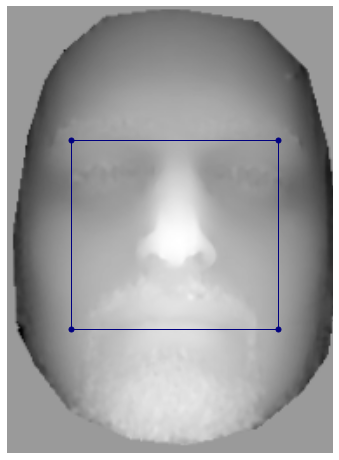
\includegraphics[width=\textwidth]{statistical_normals/images/lk2d/bs004_template.png}
    	\caption{Template}\label{subfig:singl_img_depth_2d_lk_template}
    \end{subfigure} \hfill
    \begin{subfigure}[b]{0.3\textwidth}
    	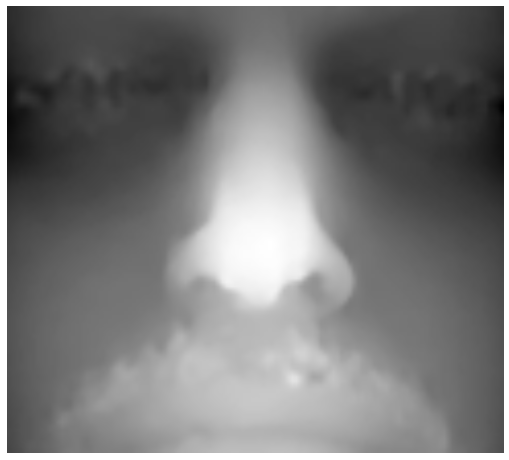
\includegraphics[width=\textwidth]{statistical_normals/images/lk2d/bs004_template_cropped.png}
    	\caption{Template Cropped}\label{subfig:singl_img_depth_2d_lk_template_cropped}
    \end{subfigure} \hfill
    \begin{subfigure}[b]{0.3\textwidth}
    	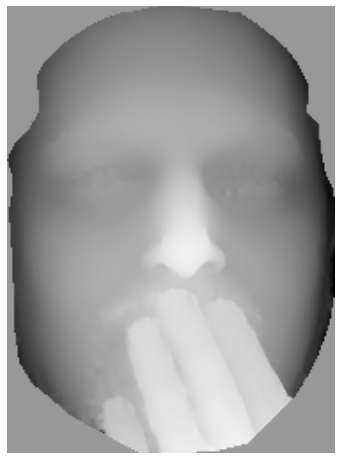
\includegraphics[width=\textwidth]{statistical_normals/images/lk2d/bs004_occluded.png}
    	\caption{Occluded}\label{subfig:singl_img_depth_2d_lk_template_occluded}
    \end{subfigure}
    \hspace*{\fill}
    \caption{An example template from the LK experiments.
             \cref{subfig:singl_img_depth_2d_lk_template_occluded} shows an
             example of an occluded image.}
\label{fig:single_img_2d_lk_examples}
\end{figure}
%%%%%%%%%%%%%%%%%%%%%%%%%%%%%%%%%%%%%%%%
%%%%%%%%%%%%%%%%%%%%%%%%%%%%%%%%%%%%%%%%
\begin{figure}[t]
    \centering
    \hspace*{\fill}
    \begin{subfigure}[b]{0.45\textwidth}
    	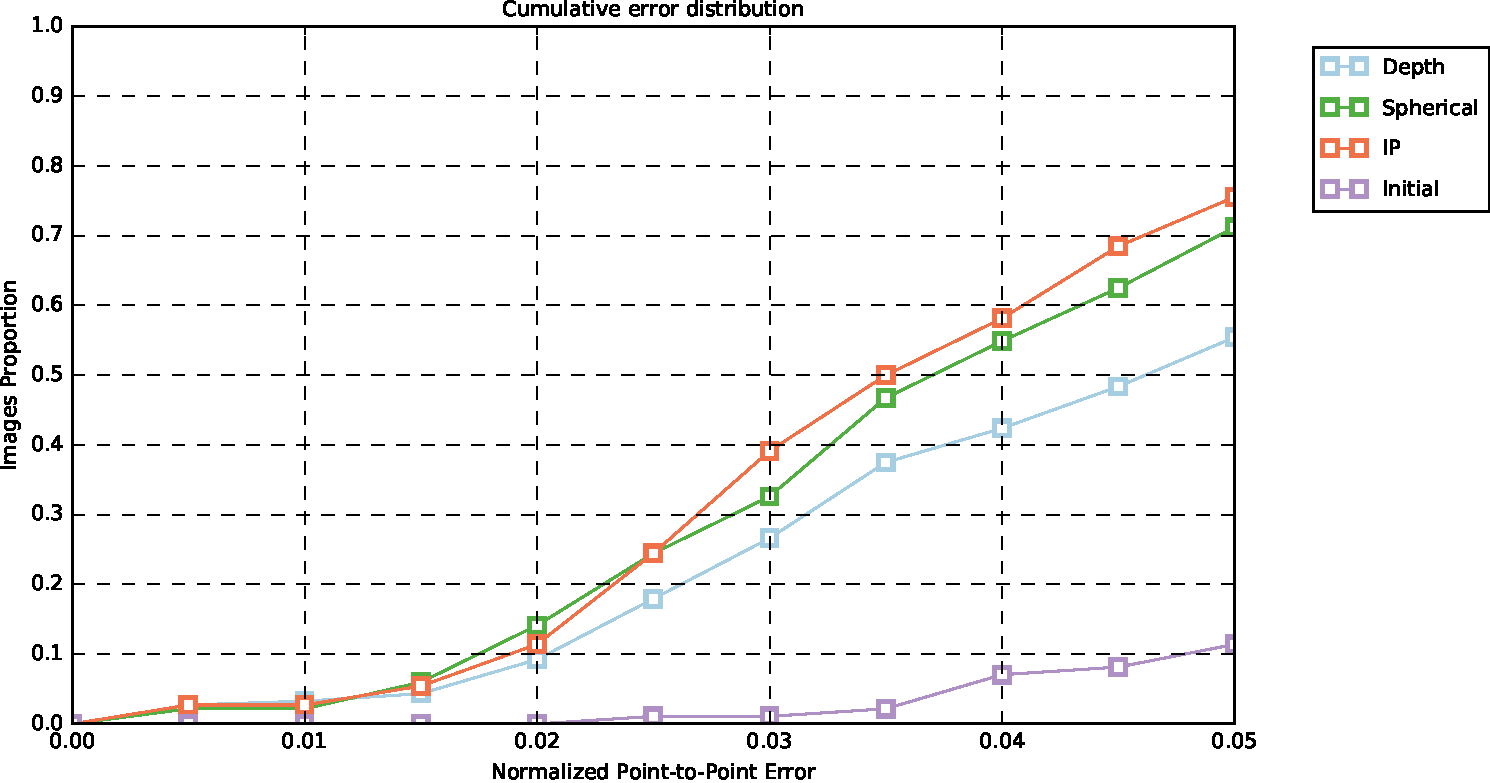
\includegraphics[width=\textwidth]{statistical_normals/images/lk2d/lk_first_5_bosphorus.pdf}
    	\caption{Uncorrupted}\label{subfig:singl_img_depth_lk_results_clean}
    \end{subfigure} \hfill
    \begin{subfigure}[b]{0.45\textwidth}
    	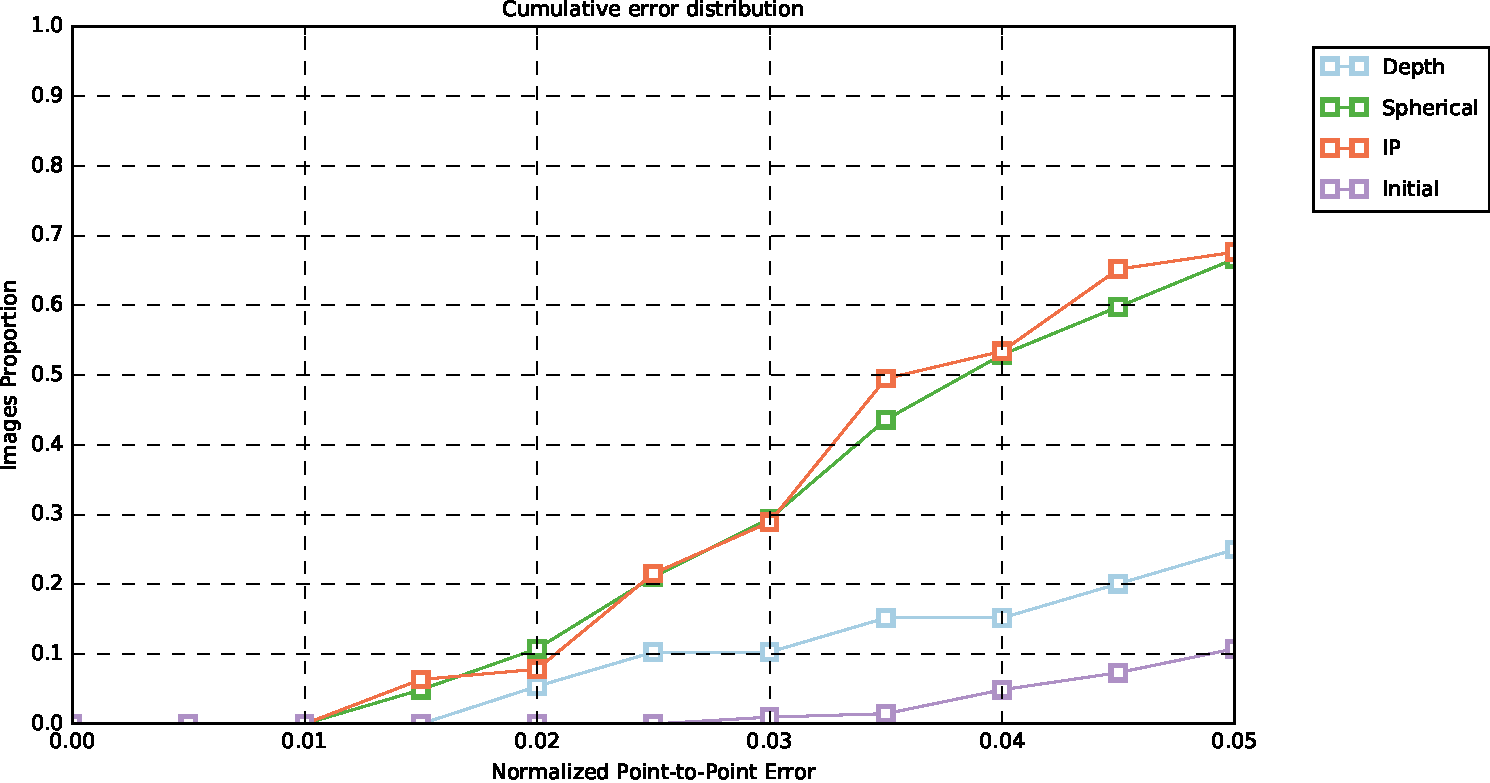
\includegraphics[width=\textwidth]{statistical_normals/images/lk2d/lk_first_5_bosphorus_dirty.pdf}
    	\caption{Occluded}\label{subfig:singl_img_depth_lk_results_dirty}
    \end{subfigure}
    \hspace*{\fill}
    \caption{Results for the Affine LK algorithms on the 
             Bosphorus~\cite{Savran:2008gg} dataset. Results are shown for the
             first 5 subjects from the database for both the uncorrupted images 
             and images containing occlusions.}
\label{fig:single_img_2d_lk_results}
\end{figure}
%%%%%%%%%%%%%%%%%%%%%%%%%%%%%%%%%%%%%%%%
%%%%%%%%%%%%%%%%%%%%%%%%%%%%%%%%%%%%%%%%
\newcommand{\aamrow}[1]{%
\adjustbox{valign=m,vspace=1pt}{\includegraphics[width=3.3cm]{statistical_normals/images/lk2d/#1_gt}}        &
\adjustbox{valign=m,vspace=1pt}{\includegraphics[width=3.3cm]{statistical_normals/images/lk2d/#1_initial}}   &
\adjustbox{valign=m,vspace=1pt}{\includegraphics[width=3.3cm]{statistical_normals/images/lk2d/#1_depth}}     &
\adjustbox{valign=m,vspace=1pt}{\includegraphics[width=3.3cm]{statistical_normals/images/lk2d/#1_ip}}        &
\adjustbox{valign=m,vspace=1pt}{\includegraphics[width=3.3cm]{statistical_normals/images/lk2d/#1_spherical}}
}

\setlength{\tabcolsep}{1pt}
\begin{figure}[t]
    \centering
    \begin{tabular}{ccccc}
        Ground Truth & Initial & Depth & IP & SPHERICAL \\ \vspace{-0.3cm}
        \aamrow{04689d98}                               \\ \vspace{-0.3cm}
        \aamrow{04708d163}
    \end{tabular}
    \caption{Examples of fitting the AAM models on the 
             FRGC v2~\cite{phillips2005overview} data. The first row shows an
             example of a failure by the depth model due to the challenging
             initialisation. The second row shows a success for the depth model
             for a simpler initialisation. Note that our normal model was
             successful in both cases.}
\label{fig:single_img_2d_aam_examples}
\end{figure}
\setlength{\tabcolsep}{6pt}
%%%%%%%%%%%%%%%%%%%%%%%%%%%%%%%%%%%%%%%%
%%%%%%%%%%%%%%%%%%%%%%%%%%%%%%%%%%%%%%%%
\begin{figure}[t]
    \centering
    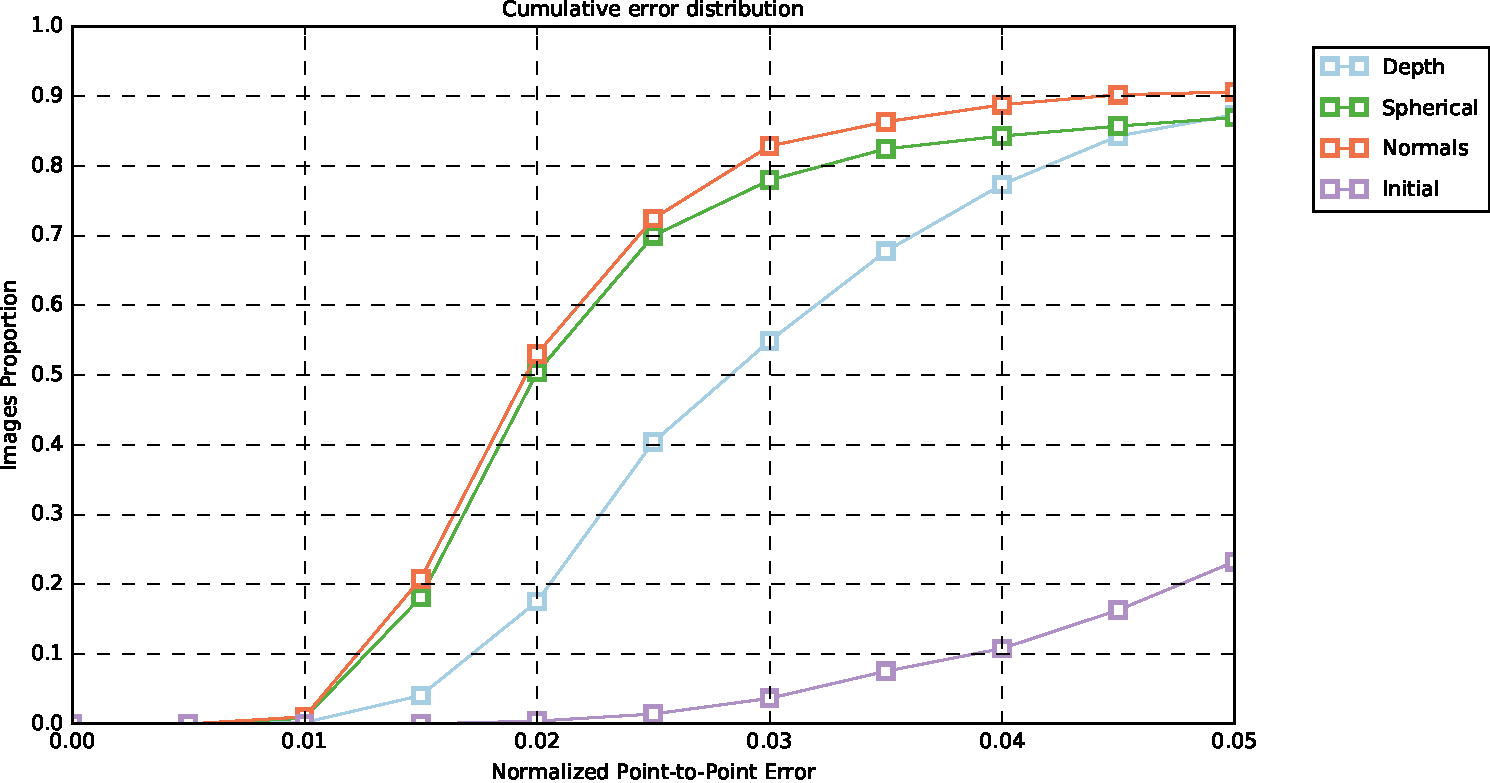
\includegraphics[width=0.7\textwidth]{statistical_normals/images/lk2d/aam_fgrc_500_random.pdf}
    \caption{Cumulative Error Distribution (CED) graph for fitting the AAM
		     models on 500 random samples from the Spring 2004 subset of the
		     FRGC v2~\cite{phillips2005overview} data. The models were trained
		     using 1000 random images from the Spring 2003 subset with no
		     overlapping identities between the training and testing data.}
\label{fig:single_img_aam_results}
\end{figure}
%%%%%%%%%%%%%%%%%%%%%%%%%%%%%%%%%%%%%%%%
%%%%%%%%%%%%%%%%%%%%%%%%%%%%%%%%%%%%%%%%
\begin{figure}[t]
    \centering
    \begin{subfigure}[b]{0.5\textwidth}
    	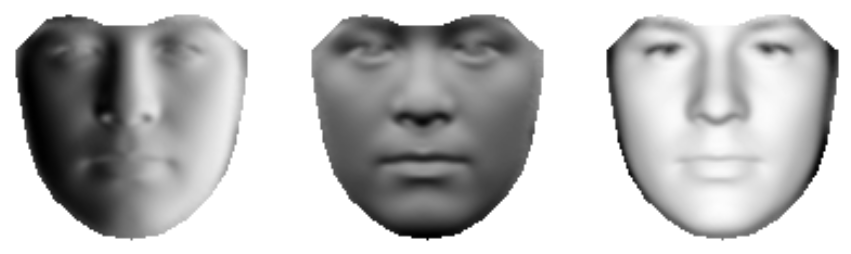
\includegraphics[width=\textwidth]{statistical_normals/images/lk2d/normals_aam_mean.png}
    	\caption{IP Mean}\label{subfig:singl_img_ip_aam_mean}
    \end{subfigure}
    \\
    \hspace*{\fill}
    \begin{subfigure}[b]{0.3\textwidth}
    	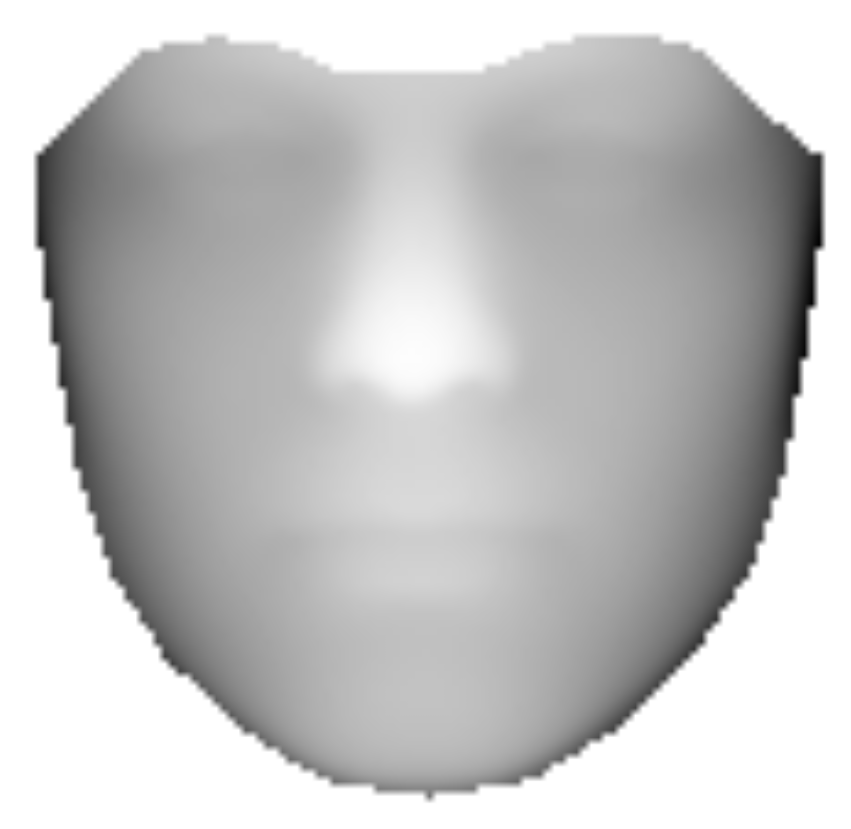
\includegraphics[width=\textwidth]{statistical_normals/images/lk2d/depth_aam_mean.png}
    	\caption{Depth Mean}\label{subfig:singl_img_depth_aam_mean}
    \end{subfigure} \hfill
    \begin{subfigure}[b]{0.3\textwidth}
    	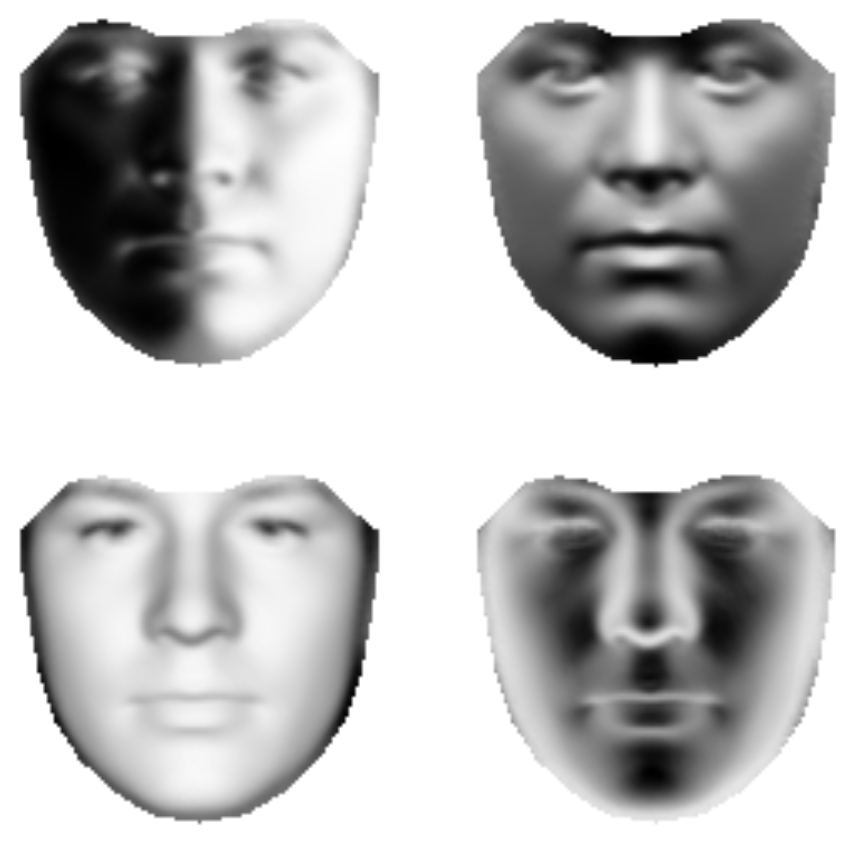
\includegraphics[width=\textwidth]{statistical_normals/images/lk2d/spherical_aam_mean.png}
    	\caption{SPHERICAL Mean}\label{subfig:singl_img_spherical_aam_mean}
    \end{subfigure}
    \hspace*{\fill}
    \caption{The appearance model means for the Depth, IP and SPHERICAL 
             AAM models.}
\label{fig:single_img_2d_aam_means}
\end{figure}
%%%%%%%%%%%%%%%%%%%%%%%%%%%%%%%%%%%%%%%%